\documentclass[10pt,a4paper]{article}
\usepackage[utf8]{inputenc}
\usepackage[english]{babel}
\usepackage[T1]{fontenc}
\usepackage{amsmath}
\usepackage{amsfonts}
\usepackage{amssymb}
\usepackage{subcaption}
\usepackage{makeidx}
\usepackage{graphicx}
\usepackage{fourier}
\usepackage{listings}
\usepackage{color}
\usepackage{hyperref}
\usepackage[left=2cm,right=2cm,top=2cm,bottom=2cm]{geometry}
\author{Tommy Müller, Marcus Dittrich, Vincent Noculak}
\title{Quadrupol-Massenfilter}


\begin{document}



\section{Theorie}

\subsection{Quadrupolfeld}

Das elektrische Potential einer Ladungsverteilung aus Punktladungen ist

\begin{equation}
	\phi(\textbf{r}) = \frac{1}{4 \pi \epsilon_0} \sum_{j} \frac{q_j}{|\textbf{r}-\textbf{r}_j|}
\end{equation}

Es kann genähert werden durch

\begin{equation}
	\phi(\textbf{r}) = \frac{1}{4 \pi \epsilon_0} \sum_{j} q_j (\frac{1}{r} + \frac{\textbf{r} \textbf{r}_j}{r^3} + \frac{3(\textbf{r}\textbf{r}_j)^2 - \textbf{r}^2 \textbf{r}^2_j}{r^5})
\end{equation}

Hier ist der erste Term der Coulomb-, der zweite der Dipol- und der dritte der Quadrupolbeitrag. Wenn die Gesamtladung und das Dipolmoment im System verschwinden, so bleibt nur der Quadrupolbeitrag übrig. Das Potential kann dann geschrieben werden als

\begin{equation}
	\phi(\textbf{r}) =  - \frac{1}{2} \phi _0 (\lambda x^2 + \sigma y^2 + \gamma z^2)
	\label{potential1}
\end{equation}

mit

\begin{align}
	\lambda = 2 Q{xx} -Q{yy}-Q{zz}\\
	\sigma = 2 Q{yy}-Q{xx}-Q{zz}\\
	\gamma = 2 Q{zz}-Q{xx}-Q{yy}\\
	Q{xx} = \frac{1}{3} \sum_{j} q_j (3 x_j^2 - r_j^2)
\end{align}

In einem ladungsfreien Raum gilt die Laplace-Gleichung($\Delta \phi = 0$) für das elektrische Potential. Für ein Quadrupolfeld, also dem Potential aus \eqref{potential1}, folgt dann

\begin{equation}
	\lambda + \sigma + \gamma = 0
\end{equation}

Diese Gleichung lässt sich mit $\lambda = - \sigma = \frac{1}{r_0^2}$ und $\gamma = 0$ lösen. Mit dieser Lösung erhalten wir das Potential

\begin{equation}
	\phi (\textbf{r}) = - \frac{1}{2} \phi _0 \frac{(x^2 - y^2)}{r_0^2}
	\label{potential2}
\end{equation}

Die Äquipotentialflächen für dieses Potentials sind Hyperbeln. Elektroden, welche die Form der Äquipotentialflächen haben, entsprechen denen eines Quadrupolmassenfilters. Der Aufbau solcher Elektroden kann in Abbildung \ref{elektrodenform} gesehen werden. Die Elektroden des von uns verwendeten Quadrupol-Massenfilters haben eine Zylinderform. Der Wert $r_0$ des Potentials ist durch den zweifachen Abstand gegenüberliegender Elektroden gegeben.

\begin{figure}[h]
	\centering
	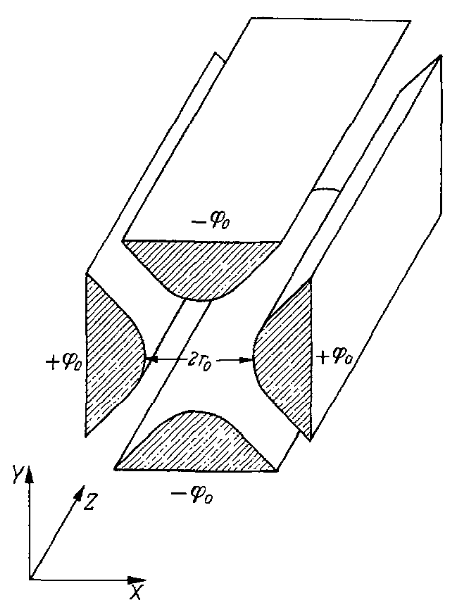
\includegraphics[scale = 0.6]{elektrodenform.png}
	\caption{Elektrodenaufbau zum Erzeugen eines Quadrupolfeldes \eqref{potential2}, Quelle: W.Paul, H.P. Reinhard und U. von Zahn, Das elektrische Massenfilter als Massenspektrometer und Isotopentrenner, 21.04.1958, S. 144}
	\label{elektrodenform}
\end{figure}

 Legt man an den Elektroden, die dieses Potentialfeld erzeugen, eine mit Gleichspannung überlagerte Wechselspannung an($\phi _0 = U + V cos(\omega t)$), so erhält man als Bewegungsgleichung eines Ions mit Masse $m$ und Ladung $Q$ in diesem Feld die Differentialgleichungen

\begin{align}
	m\frac{d^2x}{dt^2} + Q(U + V cos(\omega t)) \cdot \frac{x}{r_0^2} = 0 
	\label{xdgl1}\\
	m\frac{d^2y}{dt^2} - Q(U + V cos(\omega t)) \cdot \frac{y}{r_0^2} = 0 
	\label{ydgl1}\\
	m\frac{d^2z}{dt^2} = 0 \\
\end{align}

Aus den Gleichungen kann gelesen werden, dass es für positive Ionen bei einer reinen Gleichspannung , in x-Richtung eine rücktreibende Kraft zum Koordinatenursprung geben würde, während die Kraft in y-Richtung defokussierend wäre. Deswegen verwendet man zusätzlich eine überlagerte Wechselspannung.

Substituiert man $\omega t = 2\epsilon$, $a = \frac{8 e U}{m r_0^2 \omega^2}$ und $q = \frac{4 e V}{m r_0^2 \omega^2}$, so erhält man durch einsetzen in \eqref{xdgl1} und \eqref{ydgl1} folgende Gleichungen.

\begin{align}
	\frac{d^2x}{dt^2} + (a + 2q \cdot cos(2\epsilon)) x = 0\\
	\frac{d^2y}{dt^2} - (a + 2q \cdot cos(2\epsilon)) y = 0
\end{align}

Dies sind Mathieusche Differentialgleichungen.



\subsection{Mathieusche Differentialgleichung und Stabilitätsdiagramme}

Mathieusche Differentialgleichung sind Differentialgleichungen folgender Form:

\begin{equation}
	\frac{d^2u(x)}{dx^2} + (a + 2q \cdot cos(2x)) u = 0
\end{equation}

Für die Gleichung gibt es stabile/beschränkte und instabile/nicht beschränkte Lösungen. Ob es eine stabile Lösung gibt, ist von $a$ und $q$ abhängig. Trägt man die Bereiche für a und q, die stabile Lösungen liefern, in ein Diagramm ein, so erhält man ein sogenanntes Stabilitätsdiagramm. In Abbildung \ref{stabilitatsdiagramm1} ist ein Stabilitätsdiagramm für den Quadrupol-Massenfilter dargestellt. Der stabile Bereich hat grob die Form eines Dreiecks. Wegen $\frac{a}{q} = \frac{8 U}{4 V} = \frac{2 U}{V}$ liegen alle Ionen bei festen Spannungen auf einer Geraden. Eine solche Gerade ist exemplarisch in der Abbildung zu sehen. 

Ändert man das Verhältnis $\frac{U}{V}$, so verändert man auch die Steigung der Geraden, auf der die Ionen liegen. Folglich kann man durch das Einstellen von $\frac{U}{V}$ das Intervall stabiler q-Werte bestimmen. Weil q antiproportional zur Masse eines Ions ist, lässt sich mit dem eingestellten Wert für $\frac{U}{V}$ auch das stabile Massenintervall für Ionen einstellen. Dies macht man sich im Quadrupol-Massenspektrometer zunutze, um Ionen mit bestimmten Massen herauszufiltern. Um ein möglichst kleines Intervall von Massen zu filtern, muss die Steigung der Gerade, auf der die Ionen im Stabilitätsdiagramm sitzen, möglichst groß sein. Die Gerade muss jedoch noch den stabilen Bereich schneiden. Bei gleichbleibender Geradensteigung( Verhältnis $\frac{U}{V}$ bleibt konstant) kann man, wenn die Gerade den stabilen Bereich schneidet, die herauszufilternden Massen durch das variieren von $V$ verändern, da für ein stabilen q-Wert die dazugehörige Masse eines Ions gegeben ist durch

\begin{equation}
	m = \frac{4eV}{mr_0^2\omega^2q}
\end{equation}

\begin{figure}[h]
	\centering
	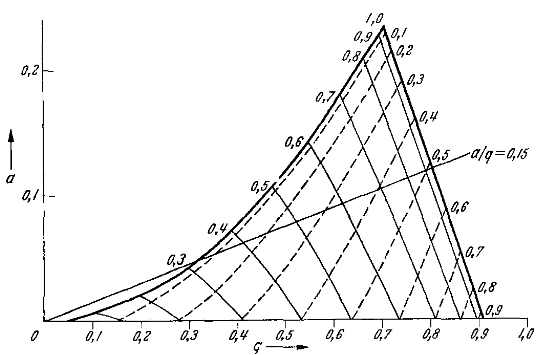
\includegraphics[scale = 0.8]{stabilitatsdiagramm.png}
	\caption{Stabilitätsdiagramm eines Quadropol-Massenfilters, Quelle: W.Paul, H.P. Reinhard und U. von Zahn, Das elektrische Massenfilter als Massenspektrometer und Isotopentrenner, 21.04.1958, S. 146}
	\label{stabilitatsdiagramm1}
\end{figure}

\subsection{Quadrupol-Massenspektrometer}

In dieser Art von Massenspektrometer werden Ionen mithilfe eines elektrischen Quadrupolfelds gefiltert. Das verwendete Quadrupolfeld entspricht dem in \eqref{potential2} und wird durch vier in z-Richtung parallel liegende Stabelektroden realisiert. Mithilfe der Stabilitätsdiagramme, die sich aus dem Lösen der Bewegungsgleichung des elektrischen Feldes ergeben, kann man zeigen, dass nur Ionen mit spezifischen Ladungen, die in bestimmten Bereichen liegen, entlang der z-Achse durch den Massenfilter gelangen können. Andere Ionen werden abgelenkt und treffen auf die Elektroden.

\subsection{Ionisierungspotential}

Das Ionisierungspotential beschreibt die Energie, die aufgewendet werden muss, um ein Molekül zu ionisieren. Die Ionisierung kann zum Beispiel dadurch verursacht werden, dass Elektronen, die durch ein elektrisches Feld beschleunigt wurden, mit einer gewissen kinetischen Energie auf ein Molekülgas treffen.

Übersteigt die Energie der Elektronen die Ionisierungsenergie des Moleküls, so kann es zusätzlich zur Ionisation in kleinere Moleküle oder atomare Bestandteile zerfallen. Haben die Zerfallsprodukte eine Gesamtladung, so erscheinen ihre Massen, wenn sie durch ein Massenspektrometer laufen, als Peaks. 

\subsection{Verwendete Gase}

\subsubsection{Argon}

Argon ist ein Edelgas mit der Ordnungszahl 18. Das am häufigsten vorkommende Isotop ist mit $99,6\%$ $^{40}$Ar, gefolgt von $^{36}$Ar mit $0,34\%$ und $^{38}$Ar mit $0,06\%$.

\subsubsection{Aceton}

Das in Abbildung \ref{aceton1} dargestellte Aceton ist das Molekül C$_3$H$_6$O. Es hat eine Masse von $58,08 \frac{g}{mol}$.

\begin{figure}[h]
	\centering
	\begin{subfigure}{0.45\textwidth}
		\centering
		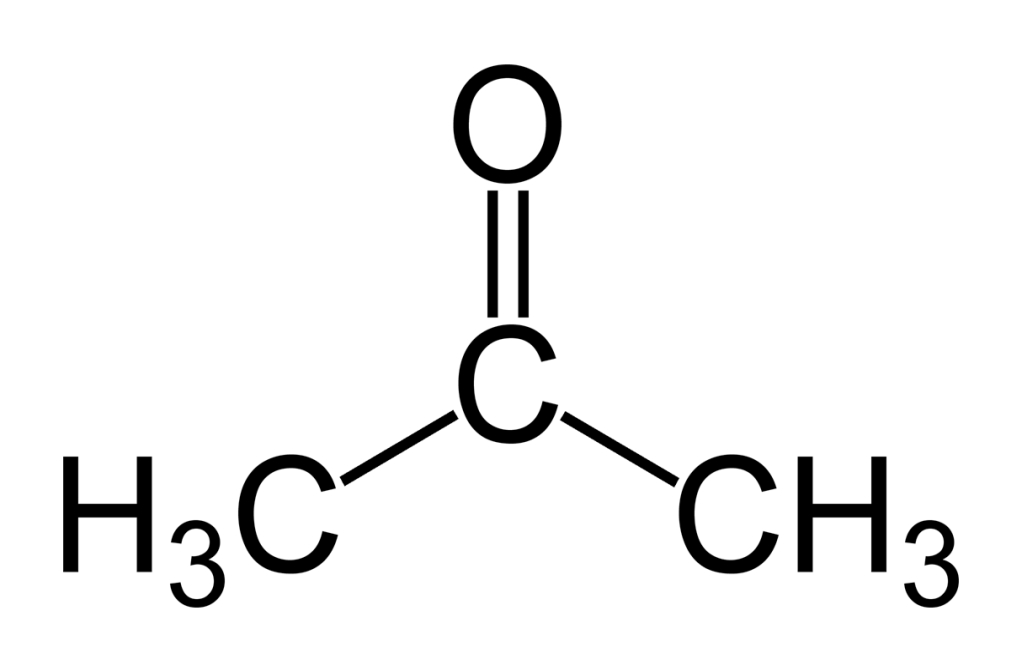
\includegraphics[scale = 0.15]{aceton.png}
		\caption{Darstellung des Aceton-Moleküls}
		\label{aceton1}
	\end{subfigure}
	\begin{subfigure}{0.45\textwidth}
		\centering
		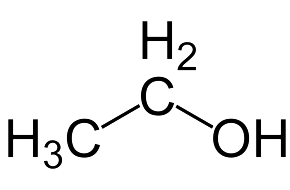
\includegraphics[scale = 0.5]{ethanol.png}
		\caption{Darstellung des Ethanol-Moleküls}
		\label{ethanol1}
	\end{subfigure}
	\caption{Im Experiment als Testgas verwendete Moleküle}
	\label{proben1}
\end{figure}

\subsubsection{Ethanol}

Ethanol(Abb. \ref{ethanol1}) ist ein einwertiger Alkohol mit der Summenformel C$_2$H$_6$O. Seine Masse beträgt $46,07 \frac{g}{mol}$.

\subsubsection{Luft}

Luft ist das Gasgemisch der Erdatmosphäre. Sie besteht zu $78,08$ Vol-$\%$ aus N$_2$(Masse: $28 u$), $20,95$ Vol-$\%$ aus O$_2$(Masse: $32u$), $0,93$ Vol-$\%$ aus Argon(Masse: $40u$) und $0,04$ Vol-$\%$ aus Kohlenstoffdioxid(Masse: $44u$). Sie enthält auch Spuren von anderen Gasen.



\section{Versuchsaufbau}

In Abbildung \ref{aufbau1} kann unser Versuchsaufbau gesehen werden. Er besteht aus einem Rezipient, in dem mithilfe zweier Vakuumpumpen ein Vakuum erzeugt wird. Dazu erreicht die Vorvakuumpumpe zuerst einen Druck von einigen Millibar. Daraufhin kann mit der Hochvakuumpumpe ein Druck im Bereich von $10^{-6} bar$ erzeugt werden. An dem Rezipient befindet sich ein Quadrupol-Massenfilter, mit dem das durch ein Dosierventil in der Rezipienten eingelassene Testgas untersucht werden kann.

Abbildung \ref{aufbau2} zeigt den inneren Aufbau des Rezipienten. Mit einer geheizten Kathode(KA) werden Elektroden freigesetzt, die durch eine Wehnelt-Elektrode(W) fokussiert als Elektronenstrahl auf das eingelassene Testgas treffen. Die Elektronen ionisieren Teile des Testgases. Das ionisierte Testgas wird auf die Eintrittsblende(EB) des Quadrupolfilters hin beschleunigt. 

\begin{figure}[h]
	\centering
	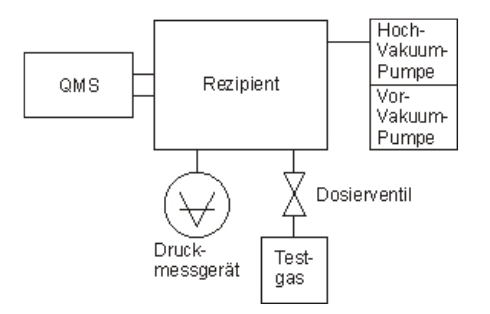
\includegraphics[scale = 0.8]{aufbau.png}
	\caption{Aufbau des Versuchs, Quelle: Anleitung der Versuchs Quadrupol-Massenspektrometer, Freie Universität Berlin}
	\label{aufbau1}
\end{figure}

\begin{figure}[h]
	\centering
	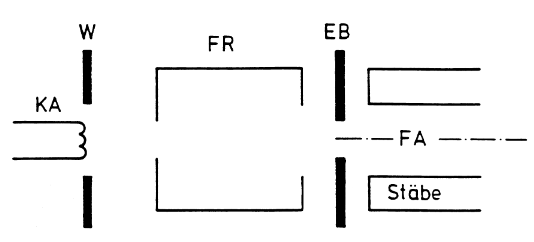
\includegraphics[scale = 0.7]{aufbau2.png}
	\caption{Innerer Aufbau des Rezipienten mit Quadropol-Massenfilter, Quelle: Anleitung der Versuchs Quadrupol-Massenspektrometer, Freie Universität Berlin}
	\label{aufbau2}
\end{figure}


\section{Durchführung}

Mit den Vakuumpumpen erzeugen wir im Rezipienten ein Vakkum im Bereich von $10^{-6} bar$. Daraufhin schalten wir den Heizdraht an. Durch das verdunsten von Wassen an der Wand der Rezipienten erhöht sich dadurch der in diesem gemessene Druck. Nachdem der Druck seinen Ausgangswert wieder erreicht hat, wird das Testgas in den Rezipienten eingelassen.

Dazu wird zunächst die Glühkathode ausgeschaltet. Das Rohr zum Zuleiten des Testgases wird zweimal mit diesem geflutet und abgepumpt, damit Rückstände eines zuvor verwendeten Testgases beseitigt werden. Daraufhin wird das Rohr erneut mit dem Gas geflutet. Mit dem Dosierventil wird das Testgas in den Rezipienten eingelassen, bis in diesem ein Druck von $1\cdot10^{-5} bar$ vorhanden ist. Nun wird die geheizte Kathode angeschaltet. Durch die dadurch stattfindende Ionisation des Testgases, kann die Messung mit dem Quadrupol-Massenfilter begonnen werden.

Das Massenspektrum wird mit Hilfe eines LabView-Programms aufgenommen. Ein Programm stellt die im Massenfilter eingestellte Gleich- und Wechselspannung automatisch ein und fährt die durchzulassenden Massenwerte automatisch in einem vorgegebenen Intervall durch. Das Labview-Programm stellt in einem Diagramm die Intensität vorgefundener Ionen gegen ihre Masse dar. Die Auflösung des Massenfilters wird voreingestellt.

Wir führen die Messung für Argon, Aceton, Ethanol und Luft durch. Das Massenspektrum von Lust nehmen wir für mehrere Auflösungen auf.

\end{document}